\section{The community detection problem}
\label{sec:ch7:comm_detect}

Throughout most of this book to date, when dealing with stochastic block models, we've assumed that we knew the community assignments ahead of time. As you learned in Section \ref{sec:ch5:psd_block:same_lp}, with networks that have an underlying block-like structure, the underlying latent positions were equal (up to a possible re-scaling by a degree-correction factor) for all nodes in the same commmunity.

When we used \texttt{ase} or \texttt{lse} to embed positive semi-definite probability matrices (and more generally, any probability matrix) in Section \ref{sec:ch6:ase} and \ref{sec:ch6:lse}, we could obtain reasonable estimates of the underlying latent position matrices (up to a rotation). We asserted, without much to back it up, that this ``latent representation'' of the adjacency matrix as a tabular structure would allow us to learn latent patterns in our network that might not necessarily be obvious at first glance, and therefore greatly simplified the conceptually complicated dependency structures that existed in our adjacency matrix. 

Let's revisit a version of our working example from Section \ref{sec:ch6:lse}, which was a network sampled from a homophilic $DCSBM_n(\vec z, \vec\theta, B)$ random network, but which has three communities instead of two. We'll also reorganize the nodes of the matrix randomly like we did in Section \ref{sec:ch6:ase:reorder}, since in many networks that you obtain, you might not be spoon-fed nodes that are pre-ordered to reflect the community structure:

\begin{lstlisting}[style=python]
import numpy as np
from graphbook_code import dcsbm

nk = 100  # 100 nodes per community
K = 3  # the number of communities
n = nk * K  # total number of nodes

zs = np.array([k for k in range(1, K + 1) for i in range(nk)])
# block matrix and degree-correction factor
B = np.array([[0.6, 0.2, 0.1], [0.2, 0.4, 0.1], [0.1, 0.1, 0.3]])
theta = np.tile(np.linspace(0, 1, nk), K)
# generate network sample
A = dcsbm(zs, theta, B)

# permute the nodes randomly
vtx_perm = np.random.choice(n, size=n, replace=False)
Aperm = A[tuple([vtx_perm])] [:,vtx_perm]
zperm = np.array(zs)[vtx_perm]
\end{lstlisting}
The network probability matrix is shown in \ref{fig:ch7:comm_detect:ex}(A), and the adjacency matrix is shown in Figure \ref{fig:ch7:comm_detect:ex}(B). Looking at the adjacency matrix, there is no obvious structure to the network.

\begin{figure}[h]
    \centering
    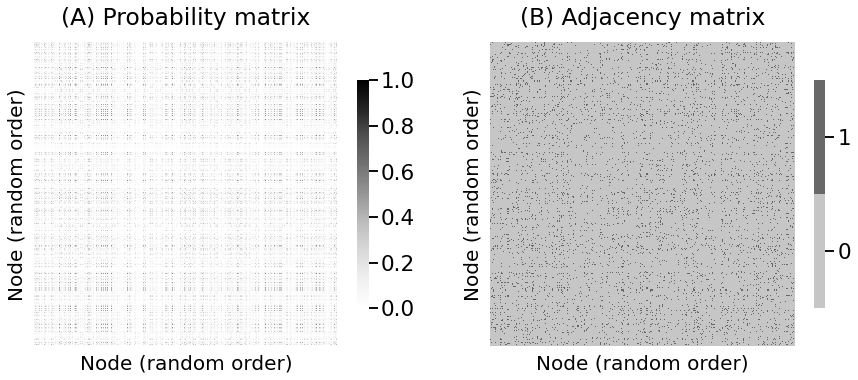
\includegraphics[width=\linewidth]{applications/ch7/Images/comm_detect_ex.png}
    \caption[Community detection three community example]{\textbf{(A)} the probability matrix for the $DCSBM_n(\vec z, \vec \theta, B)$ random networks, and \textbf{(B)} a sample of the random network.}
    \label{fig:ch7:comm_detect:ex}
\end{figure}
We would encourage you to go through the procedure of making a histogram of the node degrees to observe that the network appears to be slightly heavy-tailed, which would encourage the use of \texttt{lse}. However, for the purposes of this section, we will proceed with \texttt{ase}, as we will adjust for the elliptical-shaped latent positions using a different strategy later on. 

\begin{floatingbox}[h]\caption{Refamiliarize yourself with unsupervised learning}
In this next section, we will assume that you are familiar with several concepts from unsupervised learning, including the $k$-means algorithm, the Adjusted Rand Index (ARI), confusion matrices, and the silhouette score. If you aren't already familiar or want a quick refresher, check out the unsupervised learning basics section of the appendix in Appendix \ref{app:ch14:unsup}, which covers the required background knowledge for these concepts.

Briefly, we will use $k$-means to estimate the latent community assignment vector, the ARI and confusion matrices to study the homogeneity of the resulting latent community estimates, and the silhouette score to evaluate the latent community estimates.
\end{floatingbox}

\subsection{Spectral clustering with a pre-defined number of communities}
\label{sec:ch7:comm_detect:known}

When you embed a network with a defined number of communities, remember to use the number of embedding dimensions equal to the number of communities, because the true latent position matrix has one latent dimension for each community as you learned in Section \ref{sec:ch5:psd_block:same_lp}. In this case, since $K=3$, we embed with $3$ embedding dimensions:

\begin{lstlisting}[style=python]
import scipy as sp
from graspologic.embed import AdjacencySpectralEmbed as ase

Xhat = ase(n_components=3).fit_transform(Aperm)
D = sp.spatial.distance_matrix(Xhat, Xhat)
\end{lstlisting}
We plot the second and third embedding dimensions as a scatter plot in Figure \ref{fig:ch7:comm_detect:embed}(A), but we would encourage you to look at the entire pairs plot. Note that even though the nodes in \texttt{Aperm} were completely randomized, the estimated latent positions still retain a ``blob'' structure, where groups of nodes in the same community look spatially quite close to one another. This is reflect in the distance matrix in Figure \ref{fig:ch7:comm_detect:embed}(B), where we can see that the pairwise distances (within-community) tend to be less than the pairwise distances (between-community).


\begin{figure}[h]
    \centering
    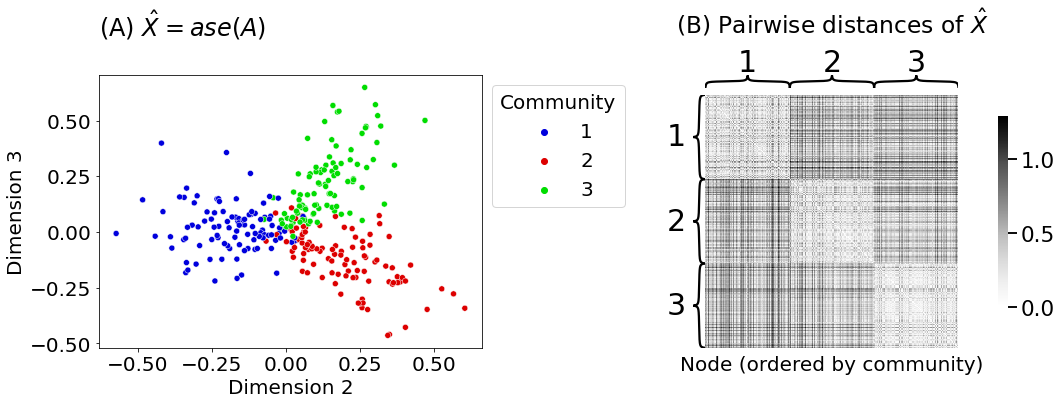
\includegraphics[width=\linewidth]{applications/ch7/Images/comm_detect_embed.png}
    \caption[Community detection spectral embedding and pairwise distances]{\textbf{(A)} a spectral embedding of the randomly ordered adjacency matrix. \textbf{(B)} the pairwise distances between the estimated latent positions for each pair of nodes.}
    \label{fig:ch7:comm_detect:embed}
\end{figure}

\subsubsection{Estimating community assignments via \texttt{KMeans}}

First, we use \texttt{KMeans} to estimate the latent community assignment vector, which we will denote with $\hat{\vec z}$. Remember that $\hat\cdot$ just means an estimate; in this case, an estimate of the community assignment vector $\vec z$ for an underlying $DCSBM_n(\vec z, \vec \theta, B)$ random network. We can produce the estimate of the community assignment vector using \texttt{KMeans()} from \texttt{sklearn}:

\begin{lstlisting}[style=python]
from sklearn.cluster import KMeans

labels_kmeans = KMeans(n_clusters = 3).fit_predict(Xhat)
\end{lstlisting}

One slight problem with this procedure is that, by being fully unsupervised, there is no reason that the labels that we estimate will necessarily ``align'' with true descriptors (such as communities) with the nodes. For instance, in this case, we have no reason to believe, for instance, that community $1$ produced by \texttt{KMeans} will necessarily correspond to community $1$ in our network. For this reason, we need to get a bit creative when evaluating unsupervised clustering techniques.

\paragraph{Evaluating your clustering}
\label{ch7:comm_detect:eval}

In this instance, you have your true community labels already known, because this is just a simulation. When you know true node labels ahead of time, you can do some special evaluations that take advantage of the fact that you have the true labels. The first of these is to study the confusion matrix, which you can produce with \texttt{sklearn}'s \texttt{confusion\_matrix()}:

\begin{lstlisting}[style=python]
from sklearn.metrics import confusion_matrix

# compute the confusion matrix between the true labels z
# and the predicted labels labels_kmeans
cf_matrix = confusion_matrix(zperm, labels_kmeans)
\end{lstlisting}

The confusion matrix is shown in Figure \ref{fig:ch7:comm_detect:eval}(A). When you have a good clustering that aligns well with your true labels, you will see that the predictions will tend to be homogeneous: a particular true label will correspond to a particular predicted label, and vice-versa. You can evaluate this homogeneity (how well, in general, one true label corresponds to one predicted label, and vice-versa) using the Adjusted Rand Index (ARI), where a score of closer to $1$ indicates that the true and predicted labels are perfectly homogeneous (one true label corresponds to exactly one predicted label):

\begin{figure}[h]
    \centering
    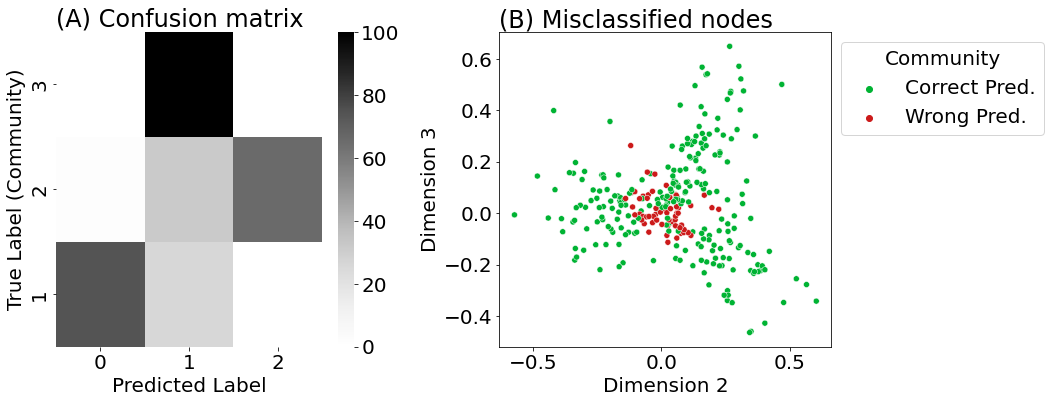
\includegraphics[width=\linewidth]{applications/ch7/Images/comm_detect_eval.png}
    \caption[Community detection clustering evaluation]{\textbf{(A)} the confusion matrix. \textbf{(B)} the estimated latent positions, along with whether the node was classified correctly (or not) after realigning the predicted communities with the true communities.}
    \label{fig:ch7:comm_detect:eval}
\end{figure}

\begin{lstlisting}[style=python]
from sklearn.metrics import adjusted_rand_score

ari_kmeans = adjusted_rand_score(zperm, labels_kmeans)
print(ari_kmeans)
# 0.4687
\end{lstlisting}
This score of about $0.5$ indicates that the predicted communities tend to be relatively homogeneous with the true labels, but the clustering is imperfect.


\paragraph*{By remapping the labels, we can evaluate the error rate}

Looking back at the confusion matrix in Figure \ref{fig:ch7:comm_detect:eval}, it looks like we have a pretty reasonable pattern we can establish:
\begin{enumerate}
    \item Nodes that are assigned a predicted label of $0$ tend to correspond to community $1$, 
    \item Nodes that are assigned a predicted label of $1$ tend to correspond to community $3$, and
    \item Nodes that are assigned a predicted label of $2$ tend to correspond to community $2$.
\end{enumerate}
It seems pretty clear that this would make for a reasonable \textit{correspondence} between the predicted and true labels. A \textit{correspondence} between two sets (in this case, the predicted and true labels for node communities) refers to the fact that we can define a mapping that relates the elements of the predicted labels to the true labels. 

When the results are not as homogeneous as they are here, this can be quite finnicky, so we will avoid going into too much depth in this book. We can remap the labels with \texttt{graspologic}'s \texttt{remap\_labels()} utility:

\begin{lstlisting}[style=python]
from graspologic.utils import remap_labels

labels_kmeans_remap = remap_labels(zperm, labels_kmeans)
\end{lstlisting}
With the labels from \texttt{KMeans} properly aligned to the true community labels, we can evaluate the error rate of our function. You can do this with \texttt{numpy} like this:

\begin{lstlisting}[style=python]
# compute which assigned labels from labels_kmeans_remap differ from the true labels z
error = z - labels_kmeans_remap
# if the difference between the community labels is non-zero, an error has occurred
error = error != 0
er_rt = np.mean(error)  # error rate is the frequency of making an error
\end{lstlisting}

In Figure \ref{fig:ch7:comm_detect:eval}(B), we visualize the misclassified points as a function of the data matrix that is being leveraged to estimate community assignments, the estimated latent position matrix. Notice that we do a good job of classifying points in the ``arms'' of the individual blobs of nodes (the \textit{clusters}), and tends to do worse for the points that are located between the clusters of nodes. This is a function of the manner in which predicted community labels are applied by \texttt{KMeans}. See Remark \ref{box:ch7:kmeans_for_sc} and Appendix \ref{app:ch14:unsup} for more detailed commentary on why this is the case.

\begin{floatingbox}[h]\caption{Why does \texttt{KMeans} perform well for clustering samples of block models?}
\label{box:ch7:kmeans_for_sc}
When we cluster points using \texttt{KMeans}, remember that we will tend to identify clusters which reflect blobs of points in our data which have similar pairwise distances (which, in most cases, will be the pairwise Euclidean distance). Points are assigned to the cluster that they are closest to, and as the \texttt{KMeans} algorithm iterates, it attempts to identify cluster centers which minimize the cumulative pairwise distance from each pair of points to the nearest cluster. 

\,\,\,\, Remember from Section \ref{sec:ch5:psd_block:same_lp} that with stochastic block models, the underlying latent positions are identical. As we learned in Section \ref{sec:ch6:ase} the estimated latent positions tend to ``approximate'' the true latent positions. The estimates will retain this feature and the estimated latent positions will be similar (in terms of their Euclidean distance) if they are in the same community for the stochastic block model, and will tend to materialize as relatively sphere-shaped ``globs'' in the estimated latent positions. 
\end{floatingbox}

In the case of the degree-corrected stochastic block model, the underlying latent positions are identical up to a rescaling along the direction of the community-specific latent position vector. This will tend to materialize as relatively elliptical-shaped globs in the estimated latent positions along the direction of the rescaling in the underlying community-specific latent position vector. This is undesirable when we try to cluster, because \texttt{KMeans} is effectively ``penalizing'' a difference between a point and the community center symmetrically in Euclidean space. In reality, we would want the ``penalty'' to be applied asymmetrically. This motivates the use of clustering techniques which are more adaptive to rescalings along the community-specific latent position vectors, such as \texttt{GMM}, as degree heterogeneity is a common problem encountered in network data. You can explore this more in-depth by completing the exercise in Remark \ref{box:ch7:gmm}.

\begin{floatingbox}[h]\caption{Using \texttt{GMM} for clustering samples of block models}
\label{box:ch7:gmm}
Simulate from a $DCSBM_n(\vec z, \vec \theta, B)$ random network, like we did above, but skew the degree-correction vector more dramatically, with $K=2$ communities. 
\begin{enumerate}
    \item Spectrally embed the adjacency matrix into two dimensions, and illustrate that the estimated latent positions appear to be elliptical.
    \item Apply \texttt{GMM} to cluster the estimated latent positions, using \texttt{GaussianMixture} from \texttt{sklearn}. Use the techniques that we described here to evaluate the clustering procedure.
    \item Plot the community centers (the \texttt{means\_} attribute of the instantiated class) estimated by \texttt{GMM}, and plot ellipses reflecting the estimated covariance (the \texttt{covariances\_} attribute) about the community centers. You can do this by following the tutorial \cite{sklearngmm_tut}.
    \item For each point in the network, compute the probability that the point is from its assigned cluster, using the \texttt{predict\_proba()} function from the \texttt{GaussianMixture} object. Plot the estimated latent positions, with the color going from low probability (red) to high probability (green).
\end{enumerate}
Use the objective function for \texttt{GMM} to argue that this result supports that \texttt{GMM} tends to penalize points less if they are farther away from the community center but along the principal axis of the community-specific ellipse, and more if they are farther away from the community center but not along the principal axis of the community-specific ellipse. Argue why this makes sense in the context of the $DCSBM_n(\vec z, \vec \theta, B)$ random network underlying your network sample by discussing the degree-correction factor heterogeneity.
\end{floatingbox}

\subsection{Spectral clustering with an undefined number of communities}
\label{sec:ch7:comm_detect:unknown}

In real data, you almost never have a beautiful canonical modular structure that makes choosing a number of communities obvious. Further, by applying unsupervised clustering algorithms in the first place and attempting to learn community labels from your data, it's likely the case that you might not necessarily know reasonable community labels that you would expect to obtain going in. This means that it is extremely infrequently going to be the case that you know exactly how you should set the number of communities, $K$, or the number of embedding dimensions ahead of time.

\begin{floatingbox}[h]\caption{Nomenclature about clusters and communities}
With unsupervised classification, the typical nomenclature is that groups of points that are assigned to the same group by the trained classifier are called a ``cluster''. However, in our case, they are more than just clusters: they are predicted node community labels. For this reason, when we are referring specifically to the assignments themselves, we will often refer to this concept as ``predicted communities'' or something of the like. When we are referring to ``blobs of points'', we will often default to calling them clusters of points. 
\end{floatingbox}

The procedure for estimating the community assignment vector is similar to what we did previously in Section \ref{sec:ch7:comm_detect}. We again embed, but this time since we don't know the number of communities we are looking for, we will use automatic elbow selection from Section \ref{sec:ch6:dimest:dimselect}:

\begin{lstlisting}[style=python]
Xhat = ase().fit_transform(Aperm)
print("Estimated number of dimensions: {:d}".format(Xhat.shape[1]))
# Estimated number of dimensions: 3
\end{lstlisting}
Examining the pairs plot, we would again find that Dimensions 2 and 3 (as before) show fairly clearly stratified blobs in the estimated latent positions, in Figure \ref{fig:ch7:comm_detect:embed}(A). 

Since we do not know the optimal number of communities $K$ nor the true community assignments, we must choose an unsupervised clustering technique which allows us to compare clusterings with different choices of community counts. Fortunately, this is pretty easy for us to do, too, using a simple statistic known as the silhouette score, which is described in Appendix \ref{app:ch14:unsup:eval:silhouette}.

\subsubsection{Using the silhouette score to deduce an appropriate number of communities}

Using the silhouette score, deducing an appropriate number of communities is pretty easy. We choose a range of communities that we think might be appropriate for our network. Let's say, for instance, we think there might be as many as $10$ communities in our dataset. We perform a clustering using unsupervised learning for all possible numbers of communities, from $2$ all the way up to the maximum number of communities we think could be reasonable. Then, we compute the silhouette score for each number of communities. Finally, we choose the number of communities which has the highest Silhouette score. 

Let's see how to do this, using \texttt{graspologic}'s \texttt{KMeansCluster()} function:

\begin{lstlisting}[style=python]
from graspologic.cluster import KMeansCluster

km_clust = KMeansCluster(max_clusters = 10)
km_clust = km_clust.fit(Xhat_permuted)
\end{lstlisting}

To determine an optimal number of clusters, we can visualize the silhouette score as a function of the number of clusters:

\begin{lstlisting}[style=python]
import seaborn as sns
from pandas import DataFrame as df

nclusters = range(2, 11)  # graspologic nclusters goes from 2 to max_clusters
silhouette = km_clust.silhouette_ # obtain the respective silhouettes

# place into pandas dataframe
ss_df = df({"Number of Communities": nclusters, "Silhouette Score": silhouette})
sns.lineplot(data=ss_df, ax=ax, x="Number of Communities", y="Silhouette Score")
\end{lstlisting}

In Figure \ref{fig:ch7:comm_detect:kmclust}(A), we look at the number of communities as a function of the silhouette score. Notice that \texttt{KMeans} with silhouette score analysis determines that the optimal number of communities is $\hat K = 4$. 

Figure \ref{fig:ch7:comm_detect:kmclust}(B) shows the predicted communities for each node coloring the estimated latent dimensions. It appears as though \texttt{KMeans} has been ``fooled'' by the elliptical, non-spherical embeddings, and in fact determined optimal unsupervised classification performance could be achieved by adding a fourth community to the center of the estimated latent positions. This is due to the fact that \texttt{KMeans} and the silhouette score penalize all dimensions equally, which as you found in Remark \ref{box:ch7:gmm}, might not always be desirable. 

\begin{figure}[h]
    \centering
    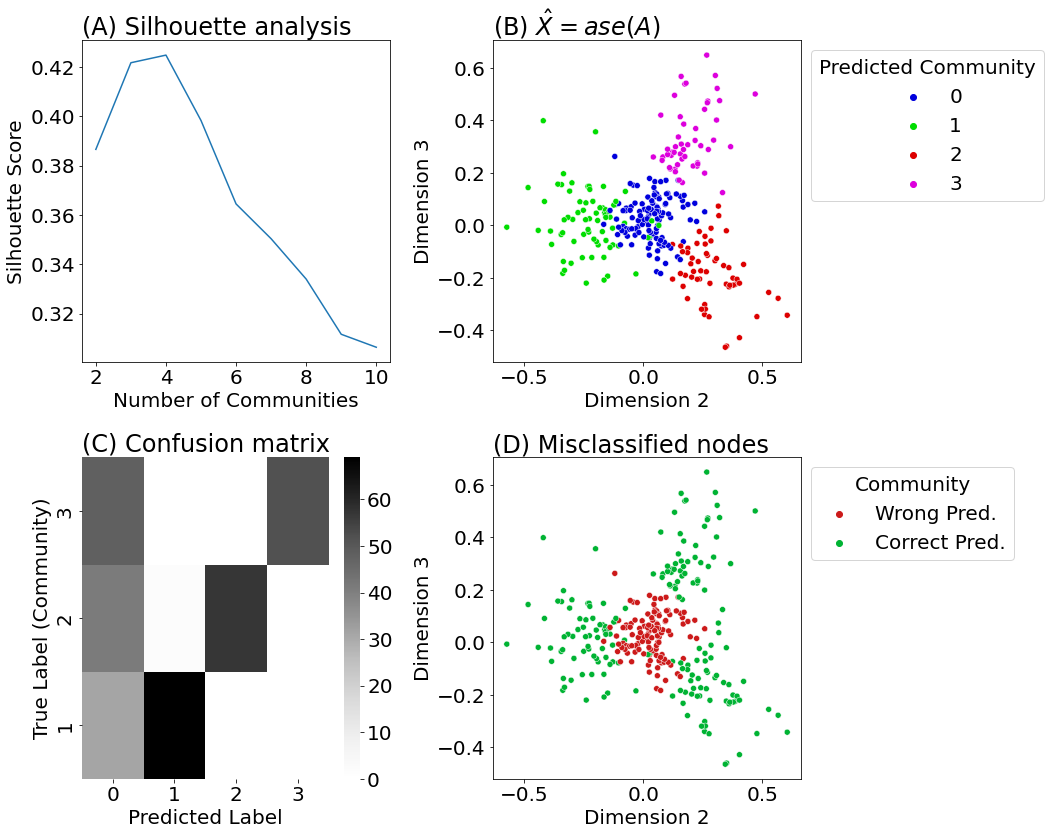
\includegraphics[width=\linewidth]{applications/ch7/Images/comm_detect_kmclust.png}
    \caption[Unsupervised community detection without knowing number of communities]{\textbf{(A)} an analysis of the silhouette scores as a function of the number of communities. \textbf{(B)} the predicted communities for each node. \textbf{(C)} the confusion matrix with $\hat K = 4$. \textbf{(D)} the misclassified points.}
    \label{fig:ch7:comm_detect:kmclust}
\end{figure}


\paragraph*{Determining what the predicted communities correspond to}

We plot the confusion matrix as a function of the true node community in Figure \ref{fig:ch7:comm_detect:kmclust}(C). The ``arms'' of the ellipses in Figure \ref{fig:ch7:comm_detect:kmclust}(B) correspond to predicted labels of $1$ through $3$ respectively, and nearly perfectly correspond with the true underlying node communities $1$ through $3$ respectively in Figure \ref{fig:ch7:comm_detect:kmclust}(C). On the other hand, the $0$ community at the center of the arms does not correspond to any particular true label particularly well, and is an agglomeration of points at the bases of the arms across all three true communities. We visualize the points that are misclassified in Figure \ref{fig:ch7:comm_detect:kmclust}(D), which correspond to the points assigned to the $0$ community. 

\paragraph*{The art of determining what predicted communities mean}

By now, you know how to apply spectral clustering to network data and evaluate it when you have a single node covariate (in this case, the true node communities). However, real data is not nearly this cut and dry: typically, associated with each node, you may have many covariates, some of which might not even have discrete (one of $K$) labels. For instance, in Figure \ref{fig:ch2:brain_preds}, for each node we had a spatial position, which would not be very easy to interpret our communities on the basis of.

For this reason, there is quite an art to determining what predicted communities mean, much like many other applications of unsupervised learning in machine learning more generally. You may have to take features that describe your nodes, such as the spatial positions listed above, and take functions of these spatial positions (such as determining the lobe of the brain that the spatial position falls into, which we described as a possible route we could take in Section \ref{sec:ch2:discover}) to be able to obtain a sensible understanding of what the communities correspond to. 

In many contexts, you might not even know what these communities correspond to at all, and you might have to rethink how the network was collected and work from the ground-up to try to find meaning in the predicted communities. In this sense, once you perform community detection and identify stable communities that appear to be well-separated, your role as a network learning scientist has really just started.

\subsection{Extending community detection to other formulations}

Algorithm \ref{alg:ch7:sc} provides a generic formulation of the community detection process for network data with adjacency representations using \texttt{KMeans} and \texttt{ase}. Note that the procedures we detail herein generalize readily to alternative approaches in which the network data can be represented as a matrix. 

\begin{algorithm}[h]
\caption{Unsupervised  spectral community detection from network data with \texttt{KMeans}}
\label{alg:ch7:sc}
\KwData{$A$ the adjacency matrix of your network.\newline $d$ Optionally, a number of embedding dimensions.\newline $K$ Optionally, a number of communities.}
\KwResult{predicted community assignments.}
\SetAlgoLined

Let $\hat X = \texttt{ase}(A, d)$. If the dimensionality $d$ is unspecified, estimate it through elbow selection in Section \ref{sec:ch6:dimest:dimselect}.

Train a \texttt{KMeans} classifier, using the representation $\hat X$, to identify $K$ communities. If the number of communities is unspecified, evaluate the classifier over a range of reasonable numbers of communities, and evaluate the clusterings using a pre-defined evaluation metric. Represent this trained classifier as the community centers $\hat{\vec \mu}_k$ for each community $k$. 

For all points, compute $d_{ik} = \|\hat{\vec x}_i - \hat{\vec \mu}_k\|_2$, or the distance from each node $i$'s estimated latent position to the community center $k$, for all communities.

Let $\hat z_i = \text{argmin}_k d_{ik}$ be the predicted community for node $i$, which is the community corresponding to the center that is closest to the estimated node latent position for node $k$.

\Return{$\hat z$}
\end{algorithm}

For instance, we could substitute \texttt{lse} for \texttt{ase}, and potentially be more robust to degree variation in the network. If we had many networks with an underlying shared structure that we wanted to learn about, we could perform \texttt{mase} on our collection of networks, and use unsupervised learning techniques to learn about the underlying shared latent position matrix. If we had particular node covariates that we wanted to incorporate into our clustering, we could use \texttt{case} to embed a weighted combination of topological network structure with node-specific covariates, and produce communities that might meaningfully inform our ability to learn from our network data. Further, we could look to non-spectral embedding techniques as well to learn latent representations about our networks. We will discuss a few in Section \ref{sec:ch10:next}.

Finally, as we covered in Remark \ref{box:ch7:gmm}, there are many unsupervised learning techniques that we could leverage (such as \texttt{GMM}) that we could use to estimate community labels from our network. If you do not specify the number of communities ahead of time and wish to evaluate a range of possible numbers of communities, it is important that you choose evaluation criteria that will reflect your choice of clustering technique. As we noted in Remark \ref{box:ch7:gmm}, \texttt{GMM} gives us flexibility in terms of degree-heterogeneities that may materialize in our embeddings. These heterogeneities made the naive Euclidean distance potentially unsuitable if our communities that we expect in our network are elliptical. However, the evaluation criteria that we used for \texttt{KMeans} (the silhouette score) uses this same Euclidean distance, and therefore might run into similar issues if used as a metric for identifying a suitable number of communities. For this reason, there might be more appropriate evaluation metrics for the particular unsupervised learning technique that you identify. In \texttt{GMM}, for instance, a popular choice is number of communities that minimizes the \texttt{BIC}.




\newpage